%%%%%%%%%%%%%%%%%%%%%%%%%%%%%%%%%%%%%%%%%%%%%%%
%Extra content for the shapefile section - but this is now being done in other chapters, and now set as an exercise.
%%%%%%%%%%%%%%%%%%%%%%%%%%%%%%%%%%%%%%%%%%%%%%%


\section{The following sections are all option practice of functionality that we have learnt in the previous chapters on the other layers}

%%%%%%%%%%%%%%%%%%%%%%%%%%%%%%%%%%%%%%%%%%%%%%%%%55
%% REMOVE TEXT IN THE MIDDLE IF HAPPY TO HAVE TIHS IN Pts SECTION
%%%%%%%%%%%%%%%%%%%%%%%%%%%%%%%%%%%%%%%%%%%%%%%%5

%\section{Attribute table}

%Each layer in the map canvas has an \textit{attribute table}. Each polygon of a layer has a row of data in the layer's \textit{attribute table}. Later in this tutorial we will be working with point data (rather than polygons) - for that layer each point will have a row of data in the layer's attribute table.

\subsection{Moving between the attribute table and the map canvas}

To open a layer's \textit{attribute table}, make sure the relative layer is highlighted in the \textit{Layers Panel}, and then click	\begin{tabular}{@{}c@{}}
\includegraphics[width=4ex]{images/attribute_table_icon.png}\end{tabular}
, or right click on layer name in the \textit{Layers Panel} and select \textit{Open Attribute Table}.

\begin{figure}[!h]
	\centering
	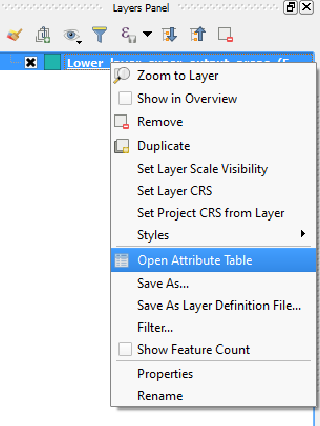
\includegraphics[width=0.25\textwidth]{images/right_click_layername_cropped.png}
	\caption{}
	\label{ft_fig_firstfig3}
\end{figure}

Can sort the data (like in excel) by clicking on the title row. Variables (columns) are referred to as \textit{fields} in GIS software. And rows as \textit{features}.\\

%Take a mental note of the fields included in this \textit{Attribute Table}. We will need to use a field that's common in both the shapefile's attribute table and a csv file that we will read in later.

\null\newpage

\subsubsection{From attribute table to map canvas}
Can select row/s in attribute table and see where they are in the map canvas (they become highlighted in yellow on the map).\\

Select top few rows (polygons) in the attribute table. Notice the \textit{Attribute table} window title reports the number of total features, and any selected.\\

\begin{figure}[!h]
	\centering
	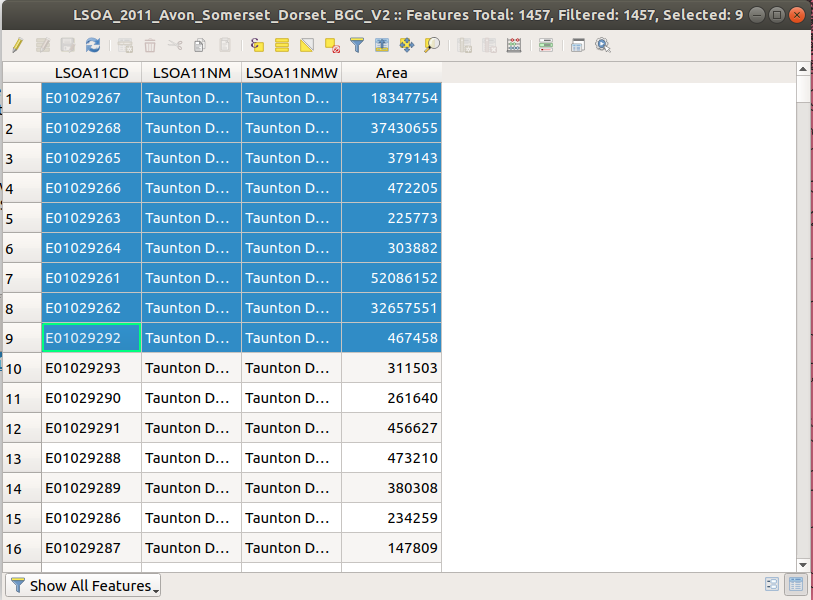
\includegraphics[width=0.6\textwidth]{images/attribute_table_top_rows.png}
	\caption{}
	\label{ft_fig_firstfig3}
\end{figure}

To know where this is on the map use the function buttons: Pan to selected, zoom to selected.

(These function buttons are in the Attributes \& Map Navigation toolbars)

\begin{figure}[!h]
	\centering
	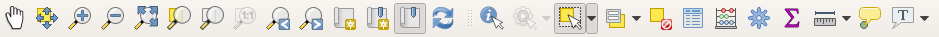
\includegraphics[width=1\textwidth]{images/attribute_and_map_navigation_toolbars_icons.png}
	\caption{}
	\label{ft_fig_firstfig3}
\end{figure}


Deselect features from all layers
	\begin{tabular}{@{}c@{}}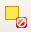
\includegraphics[width=4ex]{images/deselect_features_icon.png}\end{tabular}
and zoom full (to the shapefile layer)     
	\begin{tabular}{@{}c@{}}
\includegraphics[width=4ex]{images/full_zoom_icon.png}\end{tabular}
.

\subsubsection{From map canvas to attribute table using the \textit{Identify Feature} tool}

Click the \textit{Identify Feature} icon 
	\begin{tabular}{@{}c@{}}
\includegraphics[width=4ex]{images/identify_feature_icon.png}\end{tabular}

Click on a polygon. Information about that polygon (the values of the fields in the layer's \textit{Attribute Table}) will be displayed in the \textit{Identify Results Panel}:  

\begin{figure}[!h]
	\centering
	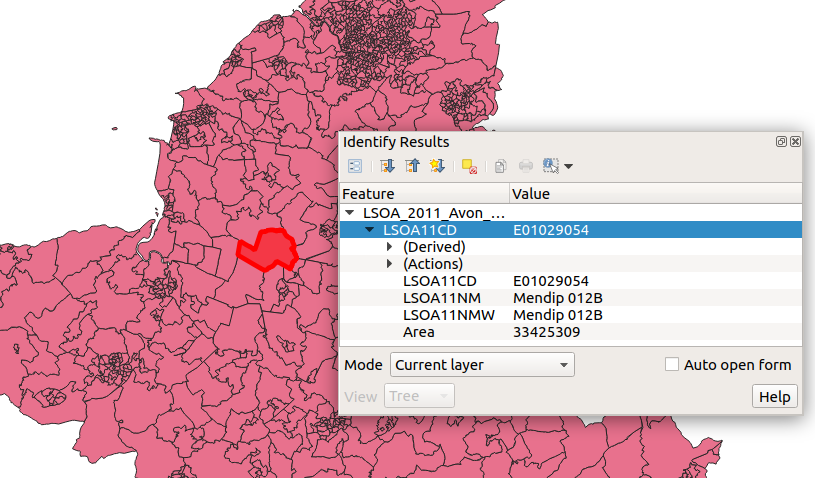
\includegraphics[width=0.6\textwidth]{images/identify_feature_window.png}
	\caption{}
	\label{ft_fig_firstfig3}
\end{figure}

\subsubsection{From map canvas to attribute table using the \textit{Select Feature(s)} tool}

Alternatively, can select multiple polygons on the map using the \textit{Select Feature(s)} tool, the icon is in the top toolbar
	\begin{tabular}{@{}c@{}}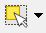
\includegraphics[width=4ex]{images/select_features_by_polygon_icon.png}\end{tabular}
, (right click to end selection) and view their field values in the \textit{Attribute Table} by moving the related rows to the top.

\begin{figure}[!h]
	\centering
	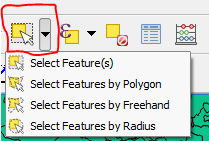
\includegraphics[width=0.35\textwidth]{images/select_features_by_polygon_dropdown.png}
	\caption{}
	\label{ft_fig_firstfig3}
\end{figure}
              
Open Attribute Table and move Selected rows to the top 
	\begin{tabular}{@{}c@{}}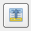
\includegraphics[width=4ex]{images/move_selection_to_top_icon.png}\end{tabular}
\null\newpage
%%%%%%%%%%%%%%%%%%%%%%%%%%%%%%%%%%%%%%%%%%%%%%%%%55
%% REMOVE TEXT IN THE MIDDLE IF HAPPY TO HAVE TIHS IN Pts SECTION
%%%%%%%%%%%%%%%%%%%%%%%%%%%%%%%%%%%%%%%%%%%%%%%%5


%%%%%%%%%%%%%%%%%%%%%%%%%%%%%%%%%%%%%%%%%%%%%%%%%55
%% REMOVE TEXT IN THE MIDDLE IF HAPPY TO HAVE TIHS IN WORLD SECTION
%%%%%%%%%%%%%%%%%%%%%%%%%%%%%%%%%%%%%%%%%%%%%%%%5

\subsection{Select features by expression}

\subsubsection{Easiest way}
The shapefile that we are working with today started as a full England and Wales shapefile that I reduced to our area of interest in order to have faster operation times. Lets go through these steps, creating an even more focused layer for just Exeter.

We can do this by using field values in the layers \textit{Attribute Table}.

Open the \textit{Attribute Table}. Click	\begin{tabular}{@{}c@{}}
\includegraphics[width=4ex]{images/attribute_table_icon.png}\end{tabular}.\\

Interrogate the data and identify which field contains data in order for us to select those that are just for Exeter.

\begin{figure}[!h]
	\centering
	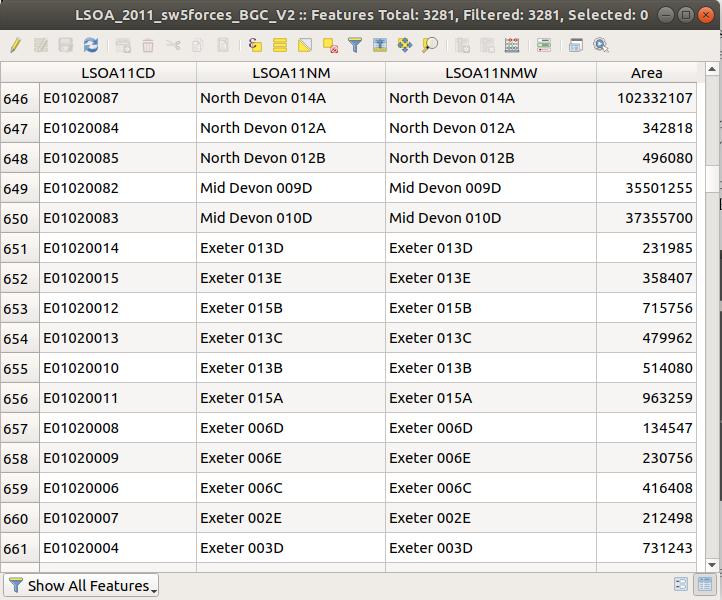
\includegraphics[width=0.35\textwidth]{images/shapefile_attribute_table.png}
	\caption{}
	\label{ft_fig_firstfig3}
\end{figure}

We have identified that field "LSOA11NM" contains the string "Exeter". So let's select those features that contain "Exeter" in that field using the \textit{Select or filter features using form}, click the icon at the top of the \textit{Attribute Table}: 
\begin{tabular}{@{}c@{}}
\includegraphics[width=4ex]{images/select_features_form_icon.png}\end{tabular}.\\

This form will help us to construct our expression to select our features.\\

Type \textit{Exeter} in the textbox relating to field "LSOA11NM"\\
From the dropdown select "Contains".\\

\begin{figure}[!h]
	\centering
	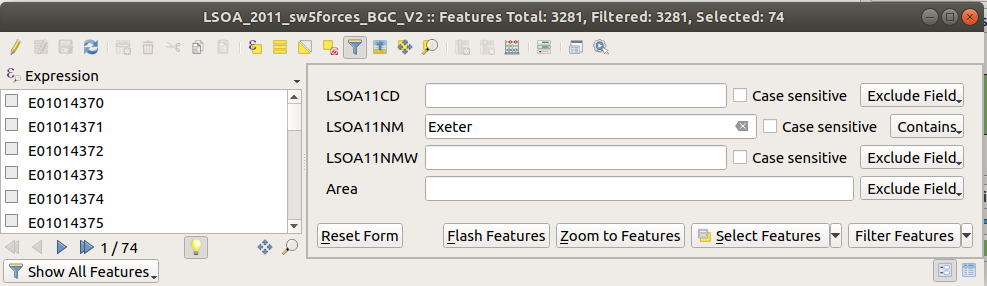
\includegraphics[width=0.8\textwidth]{images/select_filter_features_form.png}
	\caption{}
	\label{ft_fig_firstfig3}
\end{figure}

If we click the "Filter Features" button in the bottom right we can see the expression that this has built: "("LSOA11NM" ILIKE '\%Exeter\%')"\\

We can toggle between the form view and the attribute table using the buttons in the bottom right
\begin{tabular}{@{}c@{}}
\includegraphics[width=4ex]{images/form_table_icons.png}\end{tabular}. See in the \textit{Attribute Table} that 74 features exist for Exeter.\\

Let's go back to our form, click  
\begin{tabular}{@{}c@{}}
\includegraphics[width=4ex]{images/select_features_form_icon.png}\end{tabular}.\\

And now click the "Select Features" button on the bottom. Look at the map. See that Exeter is yellow (these are the selected polygons). Can zoom to them using the \textit{Zoom map to selection} icon
\begin{tabular}{@{}c@{}}
\includegraphics[width=4ex]{images/zoom_map_to_selection_icon.png}\end{tabular}.\\

\subsubsection{Alternative way}

Once we are familiar with the expressions we can type it directly in. Click the \textit{Select by expression} icon: 
\begin{tabular}{@{}c@{}}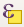
\includegraphics[width=4ex]{images/select_by_expression_icon.png}\end{tabular}.\\

And fill in the expression in the LHS pane, using the middle pane for prompts.

\begin{figure}[!h]
	\centering
	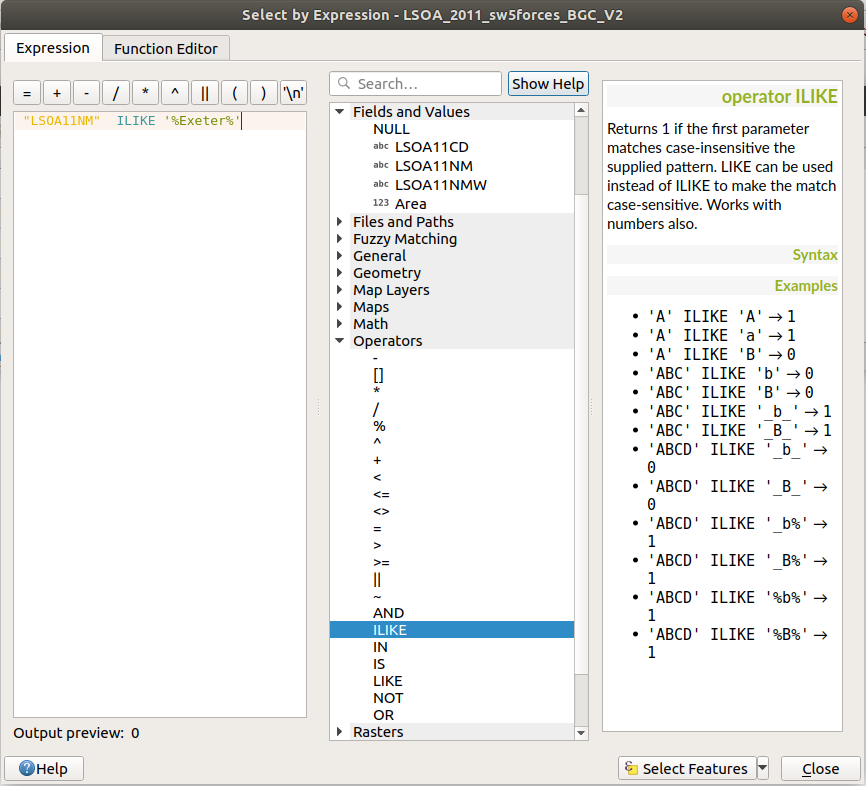
\includegraphics[width=0.8\textwidth]{images/select_by_expression_form.png}
	\caption{}
	\label{ft_fig_firstfig3}
\end{figure}

\subsection{Save selected feature as a new feature layer}
In the \textit{Layers Panel} right click on the layer's name and select Export $\rightarrow$ Save selected features as...

Type in a filename for this new shapefile. Keep "Add saved file to map" checked. Save.

\begin{figure}[!h]
	\centering
	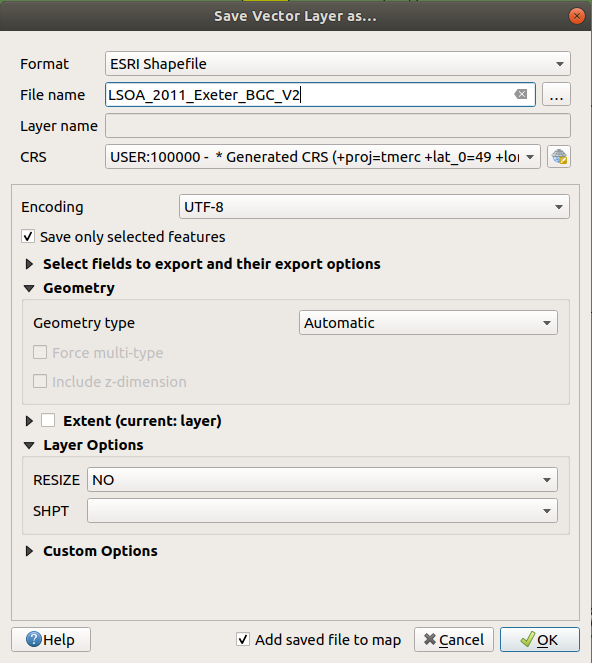
\includegraphics[width=0.6\textwidth]{images/save_vector_layer_form.png}
	\caption{}
	\label{ft_fig_firstfig3}
\end{figure}

Can see our new layer in the \textit{Layers Panel} and on the map canvas.

%%%%%%%%%%%%%%%%%%%%%%%%%%%%%%%%%%%%%%%%%%%%%%%%%55
%% REMOVE TEXT IN THE MIDDLE IF HAPPY TO HAVE TIHS IN WORLD SECTION
%%%%%%%%%%%%%%%%%%%%%%%%%%%%%%%%%%%%%%%%%%%%%%%%5


%%%%%%%%%%%%%%%%%%%%%%%%%%%%%%%%%%%%%%%%%%%%%%%%%55
%% REMOVE TEXT IN THE MIDDLE IF HAPPY TO HAVE TIHS IN LABELS SECTION
%%%%%%%%%%%%%%%%%%%%%%%%%%%%%%%%%%%%%%%%%%%%%%%%5

%\subsection{Other functionality of attribute tables}

%\begin{enumerate}
%	\item 
%	Create new fields.\\ 
%	Write expressions (formulae) to populate new fields with values (will show an example of this in the Labels Chapter). 
%	\begin{tabular}{@{}c@{}}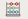
\includegraphics[width=4ex]{images/open_field_calculater_icon.png}\end{tabular}
%	\item
%	Can dock the attribute table to the main window 
%	\begin{tabular}{@{}c@{}}
\includegraphics[width=4ex]{images/dock_attribute_table_icon.png}\end{tabular}\\
%\end{enumerate}

%%%%%%%%%%%%%%%%%%%%%%%%%%%%%%%%%%%%%%%%%%%%%%%%%55
%% REMOVE TEXT IN THE MIDDLE IF HAPPY TO HAVE TIHS IN LABELS SECTION
%%%%%%%%%%%%%%%%%%%%%%%%%%%%%%%%%%%%%%%%%%%%%%%%5

%\null\newpage

%\section{Layer Properties window}

%Most of the work we will do with our layers can be initiated through the \textit{Layer Properties} window.

%To open the Layer Properties window, double click on the layer name in the Layers panel. Can also Right click $\rightarrow$ Properties (note that Right-clicking also gives many other actions for the layer, such as: remove, duplicate) 

%The LHS tabs on the Layer Properties window:

%\begin{enumerate}
%	\item
%	Information: Summary of the layer data
%	\item
%	Source: Change the Layer Name (what is used in the Layer Panel), Coordinate reference system
%	\item
%	Symbology: Stylise your layer using numerical data from the Attribute table (can also use Layers Styling panel).
%    \item
%    Labels: Add labels to the layer, using text fields from the Attribute table  (can also use Layers Styling panel).
%    \item
% 	Diagrams: Add pie chart. Text or histograms to your maps. Be careful of overcrowding your map -  only include this if your layer contains few well spaced polygons.
%	\item
%	3D view: If your data contains height information, this can incorporate it into the map. We’ve yet to use this.
%	\item
%    Source Fields: Contains the field titles of the attribute table. Currently only have data about names and areas. \textbf{We will add more data very soon and the new fields will be visible here}.
%  	\item
%	Attributes Form: We’ve yet to use this.
%	\item
%    Joins: Add spatial data to the layer. Requires a common field in both files (the layer’s Attribute table, and the new data), with a unique code for each polygon.
%	\item
%	Auxiliary Storage
%	\item
 %   Actions
%	\item
 %   Display
%	\item
%    Rendering
%	\item
%    Variables
%	\item
%    Metadata
%	\item
%    Dependencies
%	\item
%    Legend
%	\item
%    QGIS Server
%	\item
%    Digitizing
%\end{enumerate}
%
%\begin{figure}[!h]
%	\centering
%	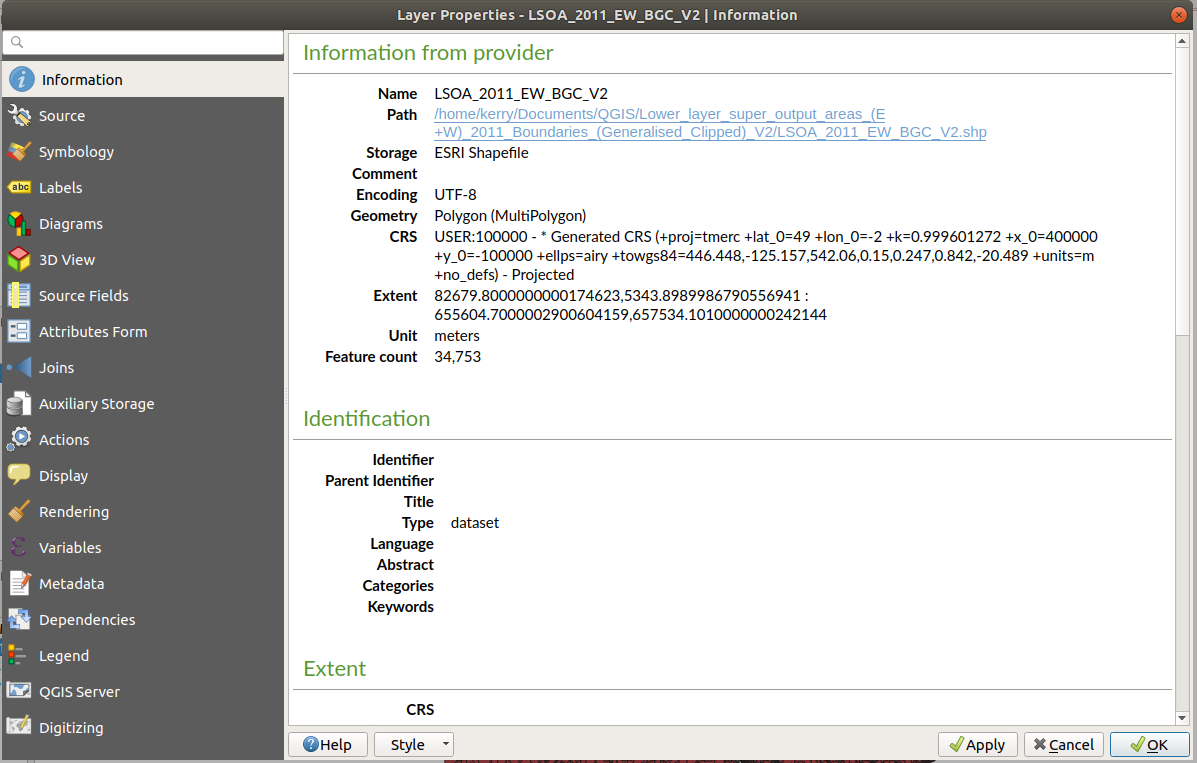
\includegraphics[width=1\textwidth]{images/layer_properties_window.png}
%	\caption{}
%	\label{ft_fig_firstfig3}
%\end{figure}

%Let's now save our project.\\

%Close QGIS and reopen. Project is present in the recent projects window, or use browse panel or menu or icon on toolbar.

%%%%%%%%%%%%%%%%%%%%%%%%%%%%%%%%%%%%%%%%%%%%%%%%%55
%% REMOVE TEXT IN THE MIDDLE IF HAPPY TO HAVE TIHS IN LABELS SECTION
%%%%%%%%%%%%%%%%%%%%%%%%%%%%%%%%%%%%%%%%%%%%%%%%5
